\documentclass[utf8]{beamer}
\usepackage [utf8]{inputenc}
\usepackage[russian]{babel}
\usepackage{caption}
\usepackage{cmap}
\usepackage[backend=bibtex]{biblatex}
\bibliography{DipBib}
\usepackage[T2A]{fontenc}
\usepackage{cmap}
\newsavebox{\longestsec}
\usetheme{Madrid}
\useoutertheme{tree}
\usepackage{epstopdf}
\usepackage{float}

\DeclareCaptionLabelFormat{andtable}{#1~#2  \&  \tablename~\thetable}


\renewcommand{\figurename}{Fig.}

\DeclareGraphicsExtensions{.eps} 

\newtheorem{mdefinition}{Определение}[section]
\newtheorem{mremark}{Примечание}[subsection]
\newtheorem{msuggest}{Предложение}[subsection]
\newtheorem{mclaim}{Утверждение}[subsection]
\newtheorem{mlemma}{Лемма}[subsection]
\newtheorem{mtheorem}{Теорема}
\newtheorem{mconseq}{Следствие}

\DeclareMathOperator{\argmax}{argmax}
\DeclareMathOperator{\argmin}{argmin}
\DeclareMathOperator{\grad}{grad}
\DeclareMathOperator{\sign}{sign}
\DeclareMathOperator{\diag}{diag}
\DeclareMathOperator{\norm}{norm}
\renewcommand{\leq}{\leqslant}
\renewcommand{\geq}{\geqslant}
\renewcommand{\phi}{\varphi}
\setcounter{figure}{0}


\title{Эксперименты по уникальности}
\date{17 мая 2017}

\institute{
 МФТИ. ФИВТ. Кафедра анализа данных \\
    \vspace{0.7cm}
    Научный руководитель:  д.ф.-м.н. Воронцов Константин Вячеславович \\
    \vspace{0.7cm}
}

\begin{document}
	\begin{frame}
		\titlepage
	\end{frame}

	\begin{frame}
		\frametitle{Краткое содержание}
		\renewcommand{\baselinestretch}{1.5}
		\fontsize{12pt}{9.2}\selectfont
		\tableofcontents
	\end{frame}
	
\section{Зависимость от коэффициента разреживания}
	\begin{frame}	
	\begin{figure}[h]
	\frametitle{Зависимость от коэффициента разреживания}
	\centering  	
	\caption{20newsgroup 3 метки. В разложении $|T| = 5$} 
	\medskip
	\includegraphics[width=0.9\linewidth]{presentation_pictures/alpha_dependency_topics_origin_3_ums.eps}  
	\end{figure}
	\end{frame}
	
	\begin{frame}	
	\begin{figure}[h]
	\frametitle{Зависимость от коэффициента разреживания}
	\centering  	
	\caption{20newsgroup 7 меток. В разложении $|T| = 10$} 
	\medskip
	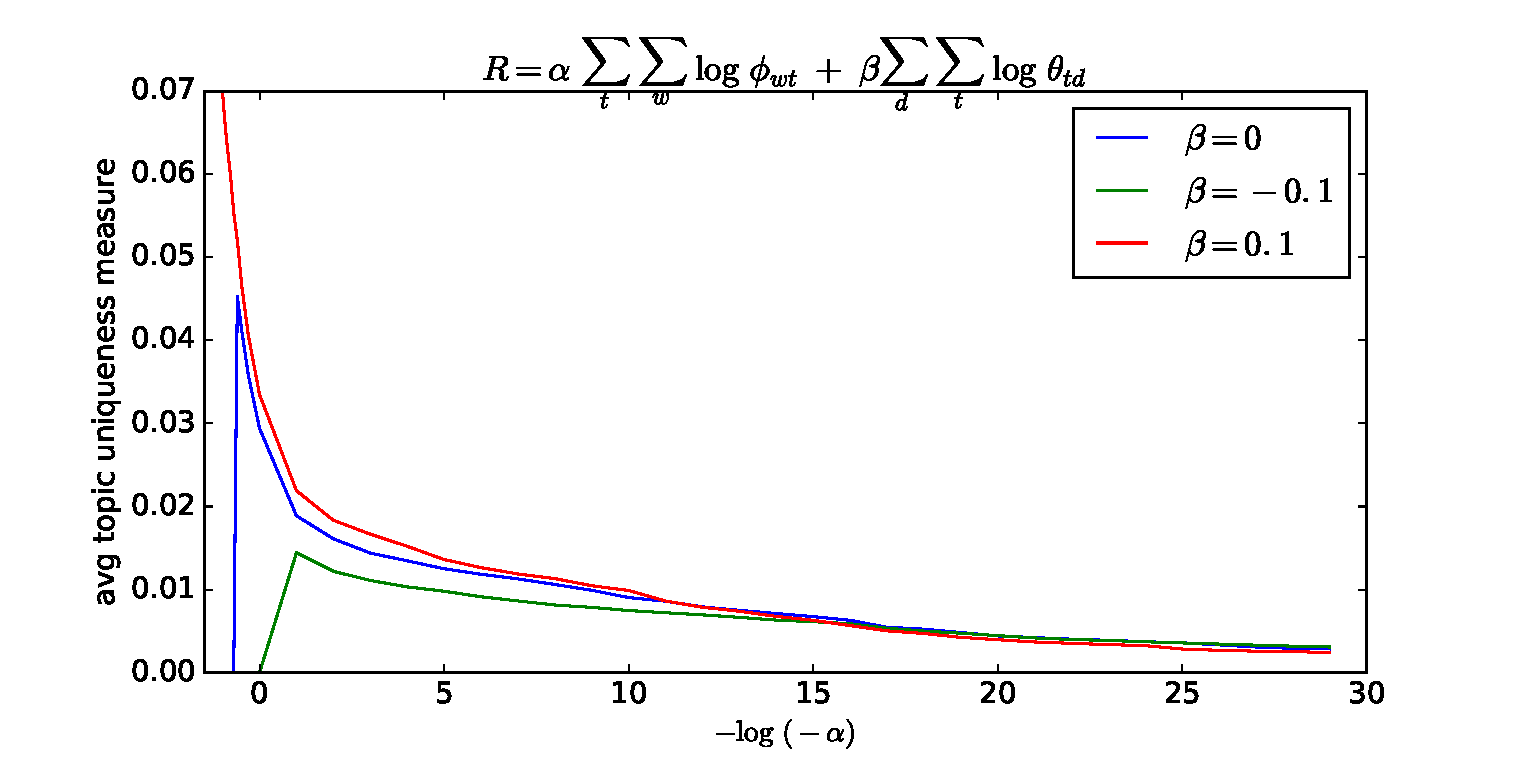
\includegraphics[width=0.9\linewidth]{presentation_pictures/alpha_dependency_topics_origin_7_ums.eps}  
	\end{figure}
	\end{frame}
	
	\section{Зависимость от числа тем}
	\begin{frame}	
	\frametitle{Описание эксперимента}
	\begin{enumerate}
\item Используем 20newsgroup с разным числом меток.
\item 10 процентов слов в каждом документе скрываем.
\item Обучаем модель на трейне и считаем меру единственности для каждой темы. Отслеживаем минимальное (по темам), максимальное и среднее.
\item У получившейся модели считаем перплексию на тесте.
\end{enumerate}
	\end{frame}
	
	\begin{frame}	
	\frametitle{Зависимость от числа тем. 1 метка}
	\includegraphics[width=0.75\linewidth]{presentation_pictures/topics_dependency_origin_1_ums.eps} 
	\end{frame}
	
	\begin{frame}	
	\frametitle{Зависимость от числа тем. 2 метки}
	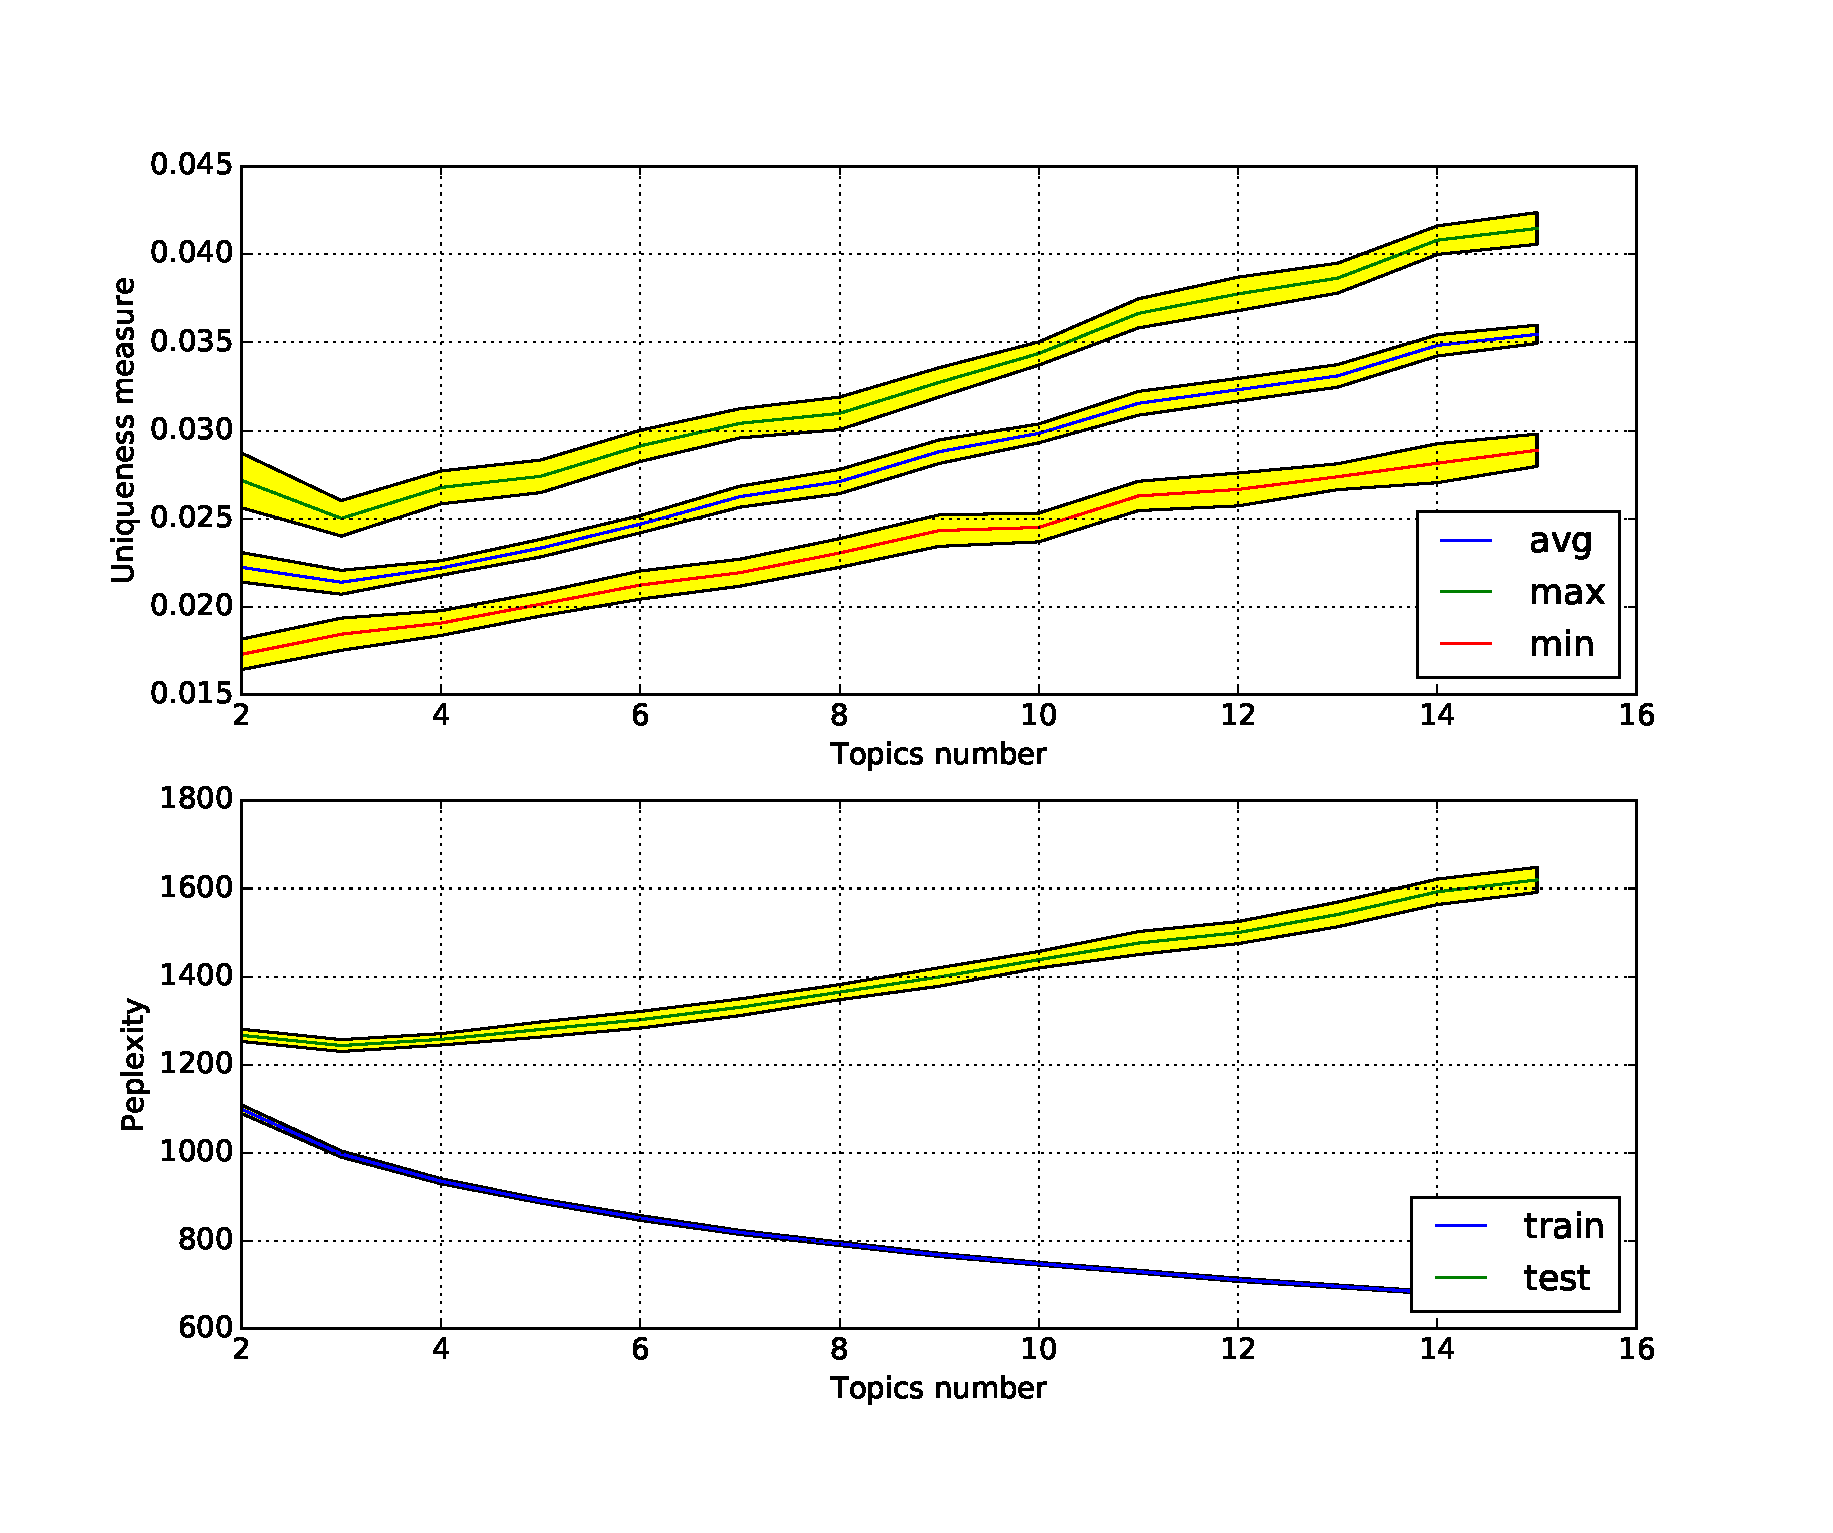
\includegraphics[width=0.75\linewidth]{presentation_pictures/topics_dependency_origin_2_ums.eps} 
	\end{frame}
	
	\begin{frame}	
	\frametitle{Зависимость от числа тем. 3 метки}
	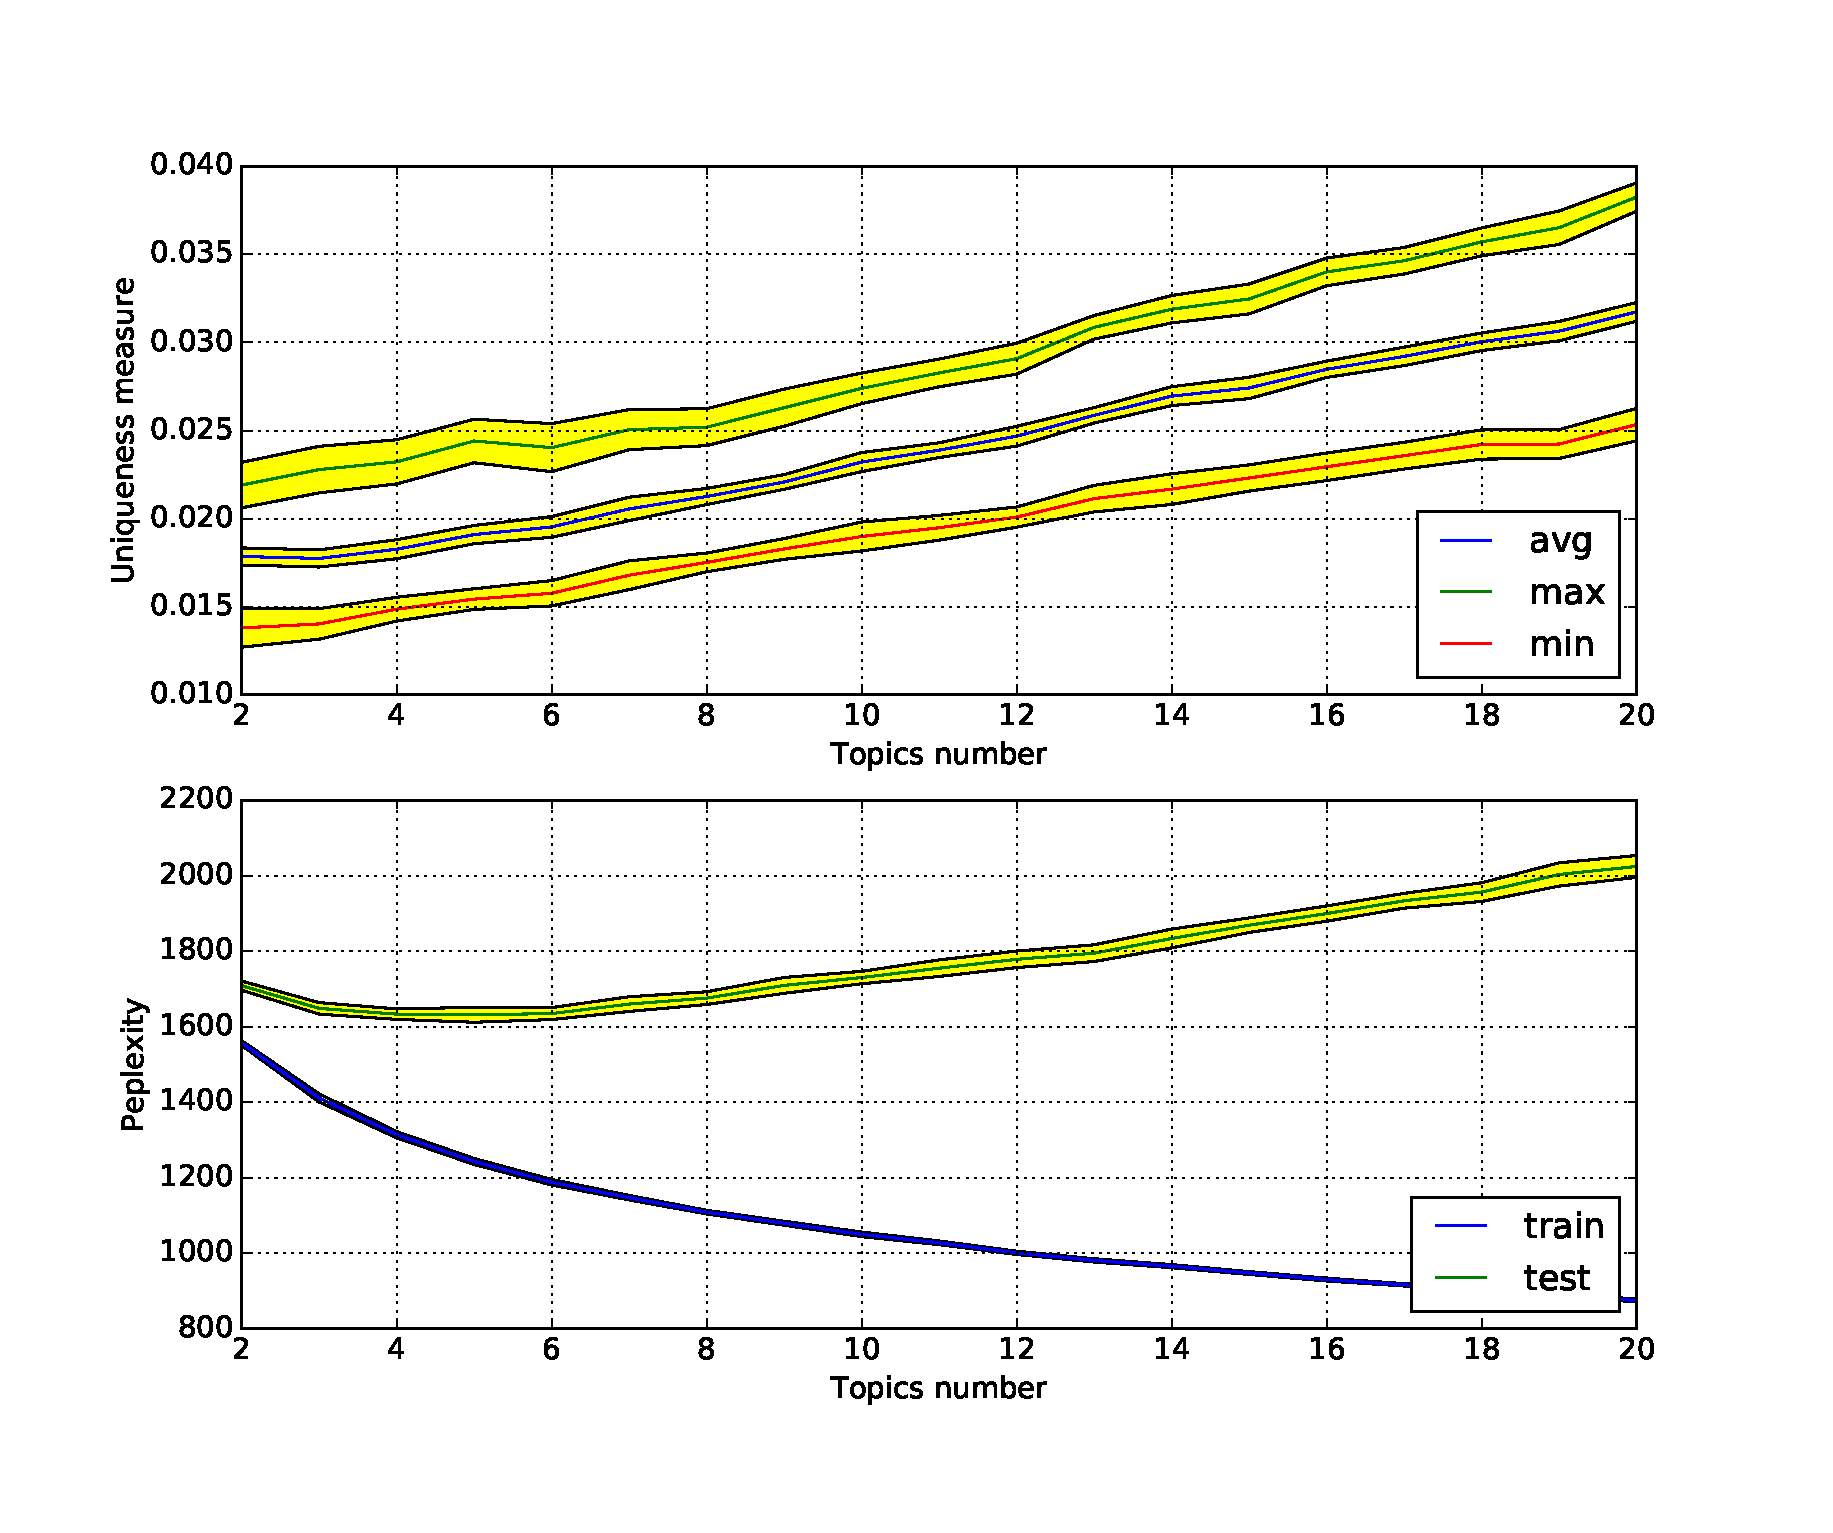
\includegraphics[width=0.75\linewidth]{presentation_pictures/topics_dependency_origin_3_ums.eps} 
	\end{frame}
	
	
	\begin{frame}	
	\frametitle{Зависимость от числа тем. 3 метки}
	\includegraphics[width=0.75\linewidth]{presentation_pictures/topics_dependency_origin_3_nums.eps} 
	\end{frame}
	
	
	\begin{frame}	
	\frametitle{Зависимость от числа тем. 4 метки}
	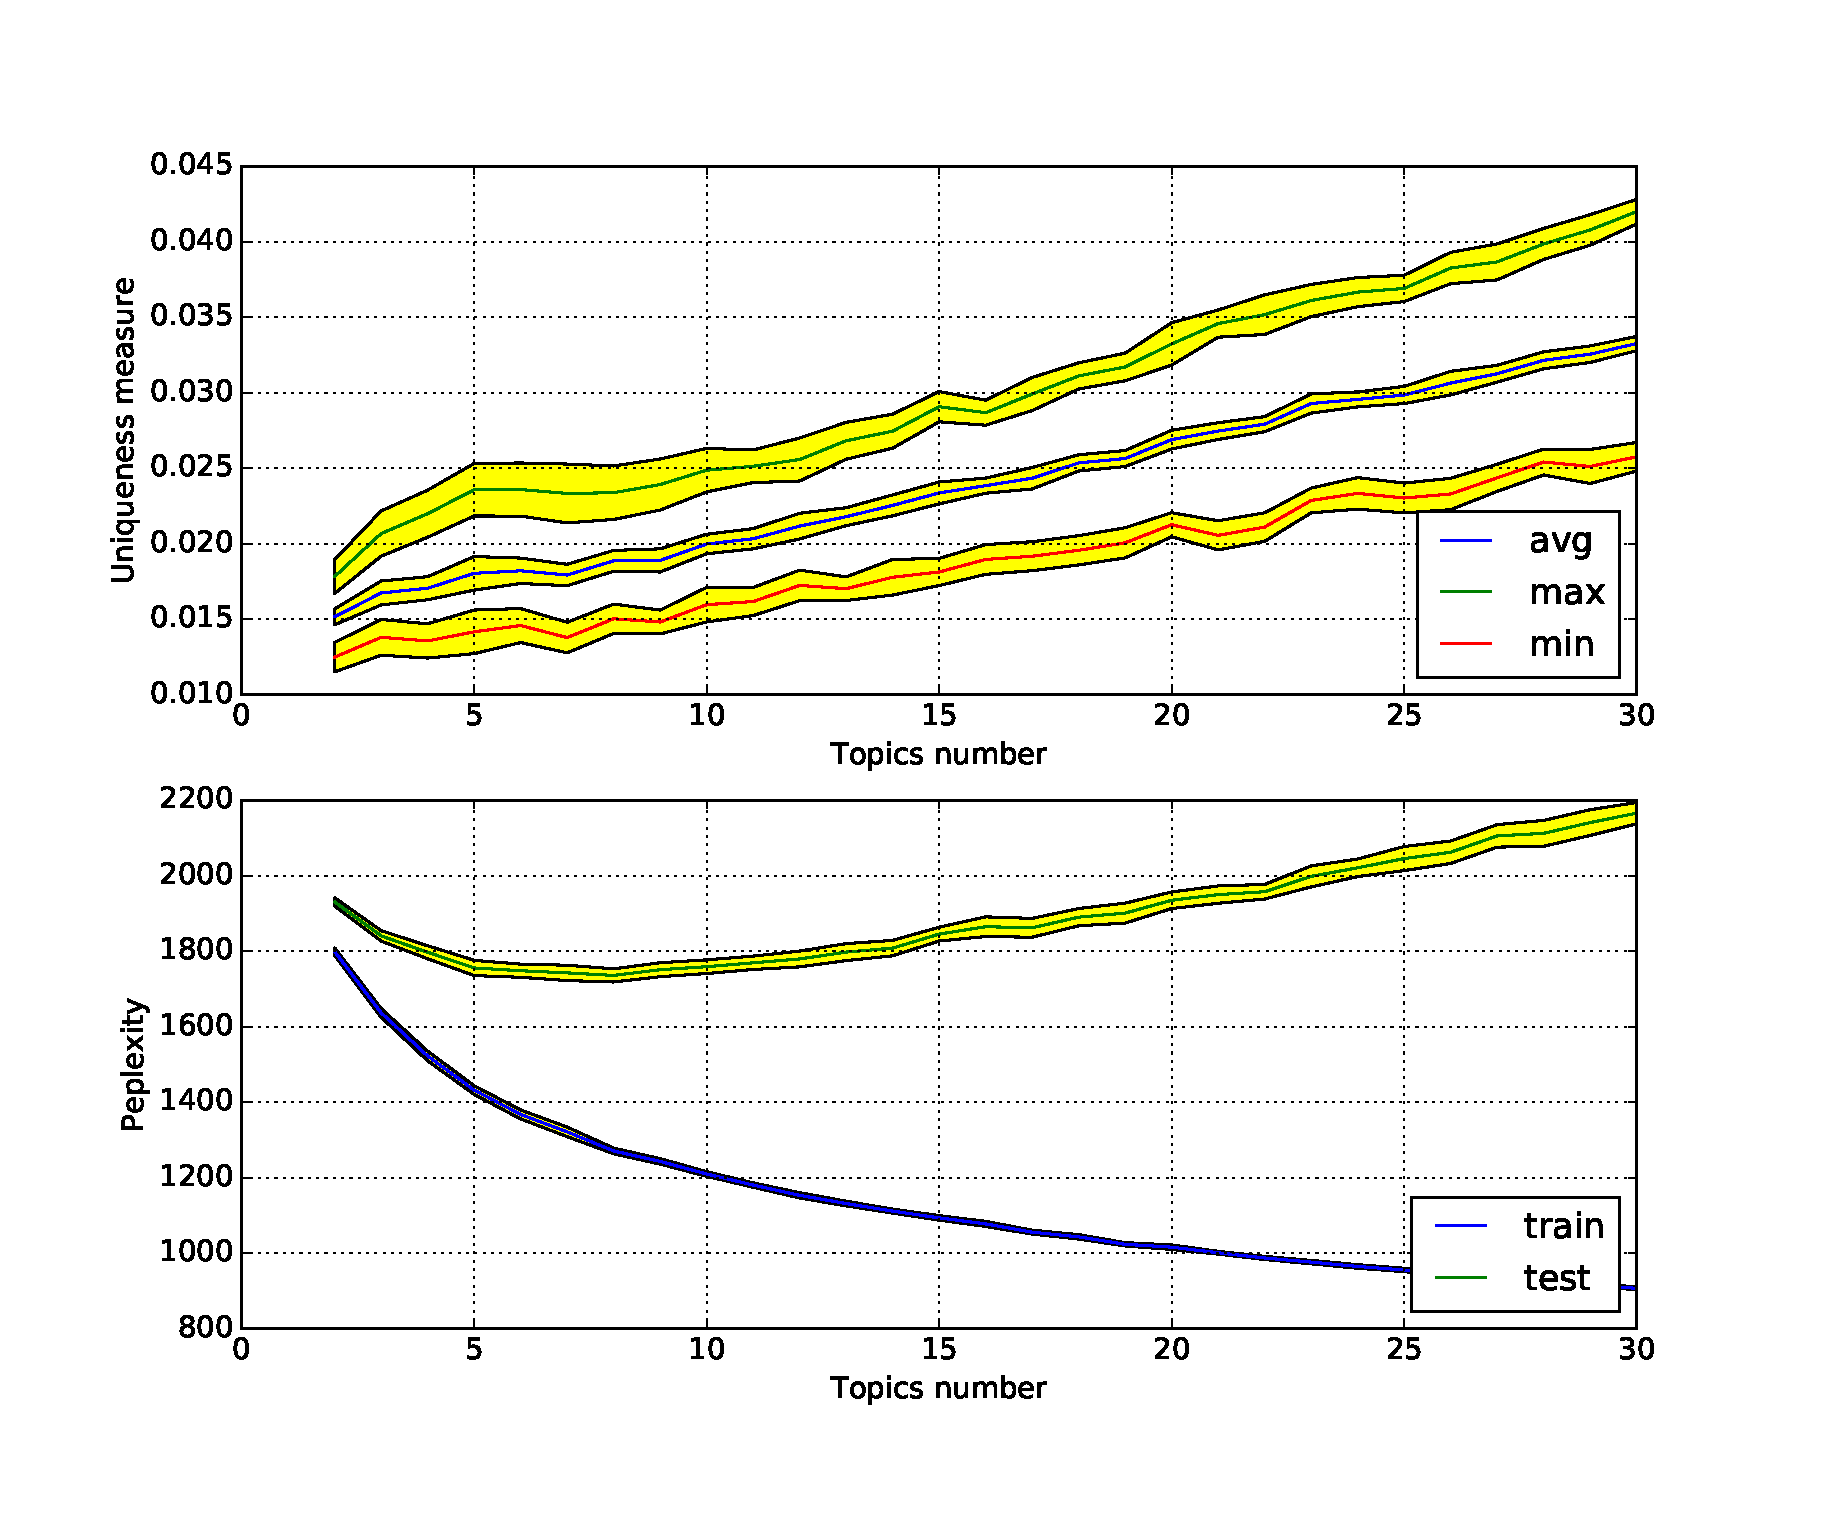
\includegraphics[width=0.75\linewidth]{presentation_pictures/topics_dependency_origin_4_ums.eps} 
	\end{frame}

	
	\begin{frame}	
	\frametitle{Зависимость от числа тем. 7 меток}
	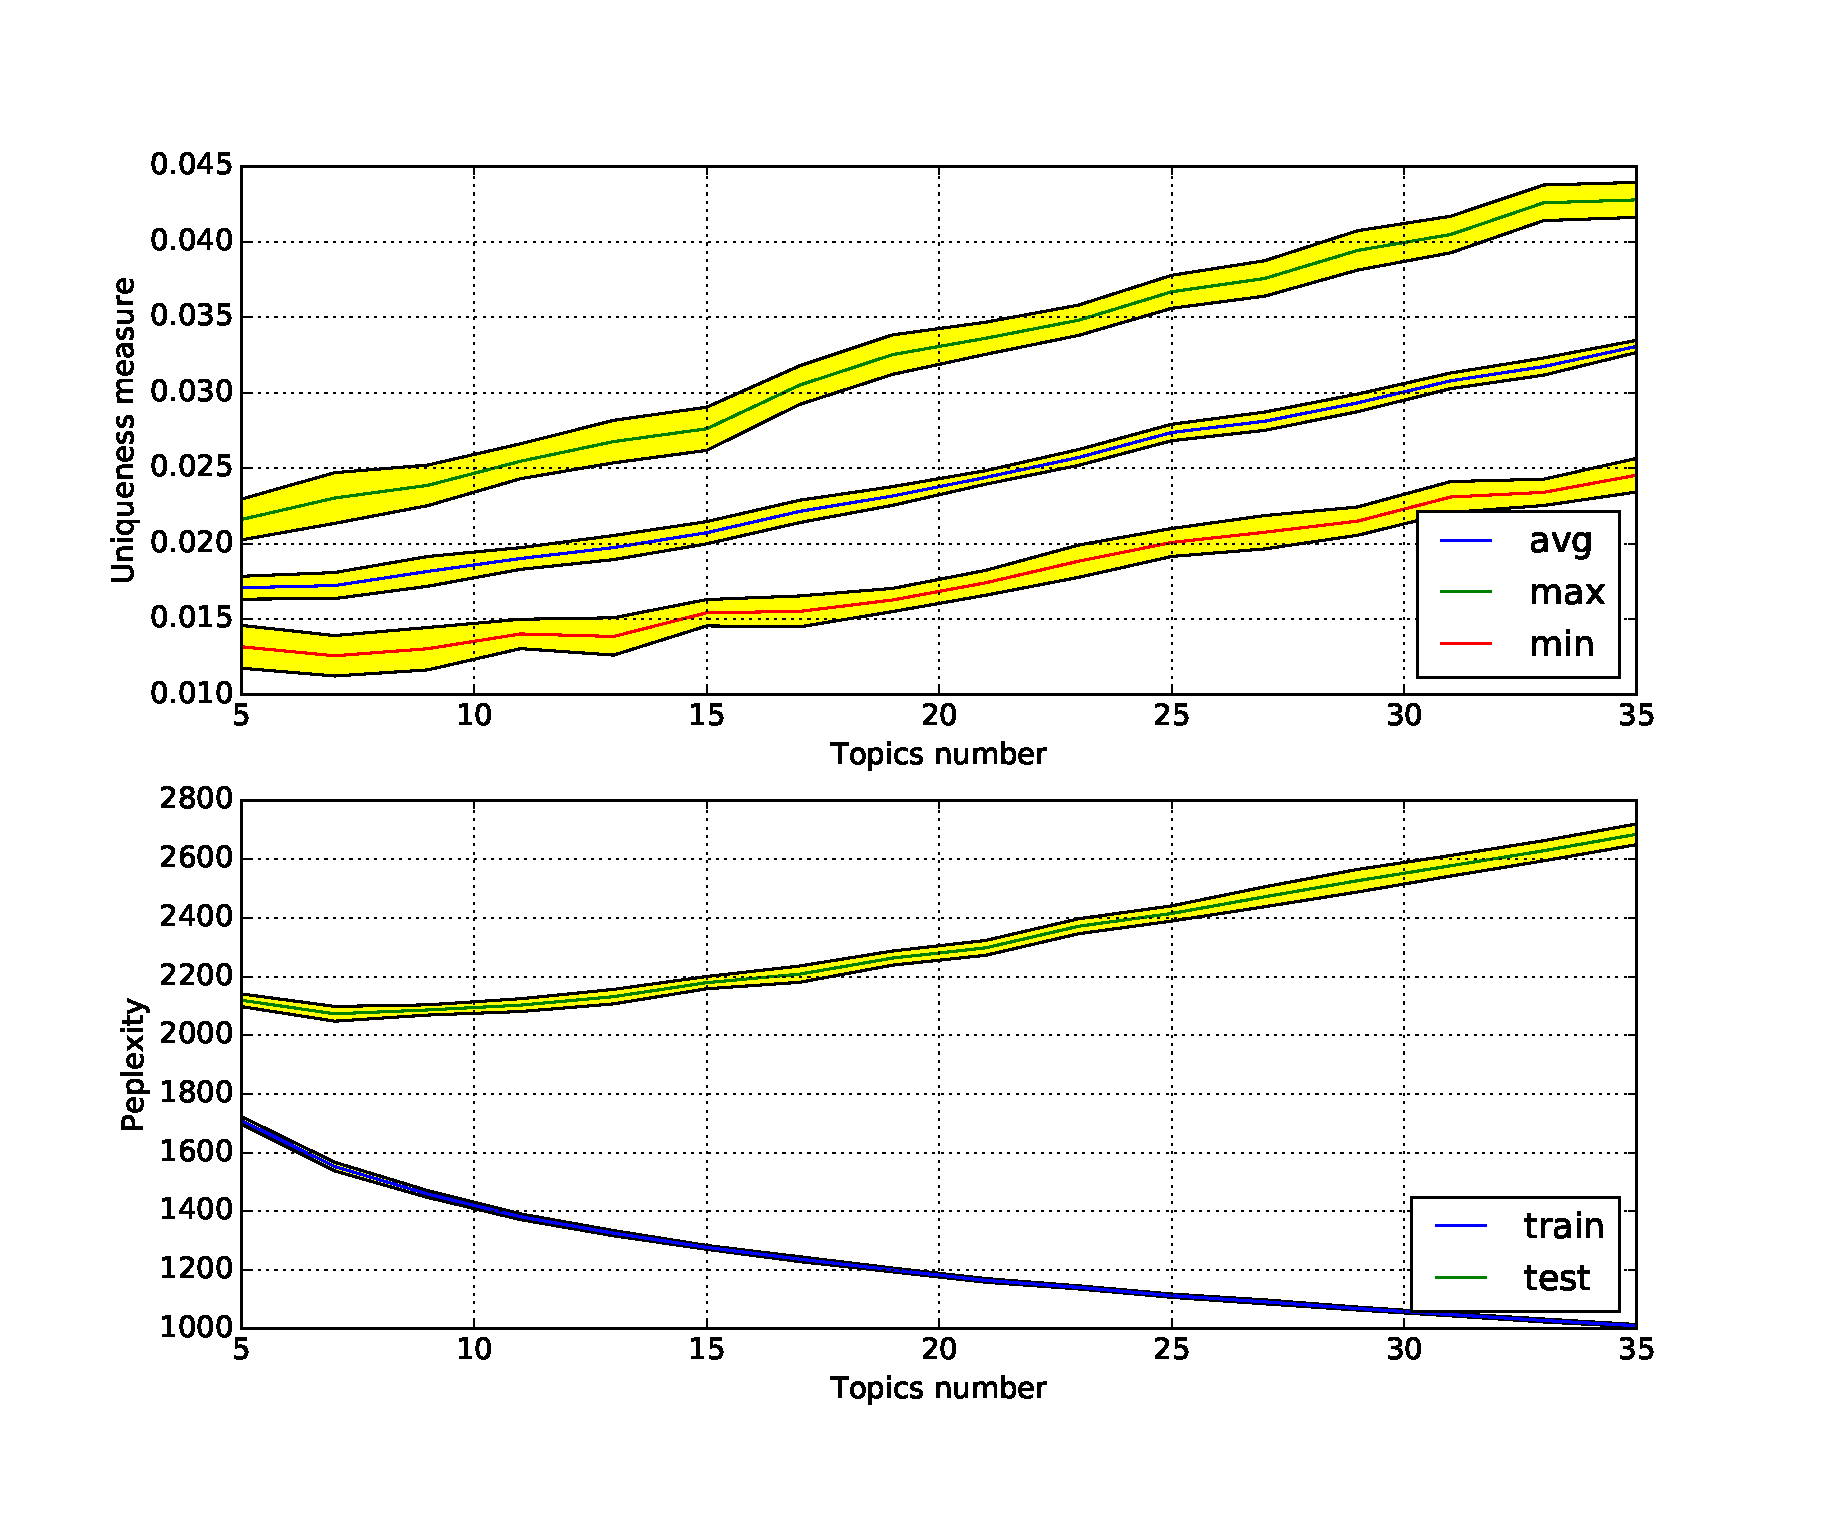
\includegraphics[width=0.75\linewidth]{presentation_pictures/topics_dependency_origin_big_ums.eps} 
	\end{frame}
	
	\section{Проверка уникальности}
	\begin{frame}	
	\frametitle{Проверка уникальности. PLSA}
	 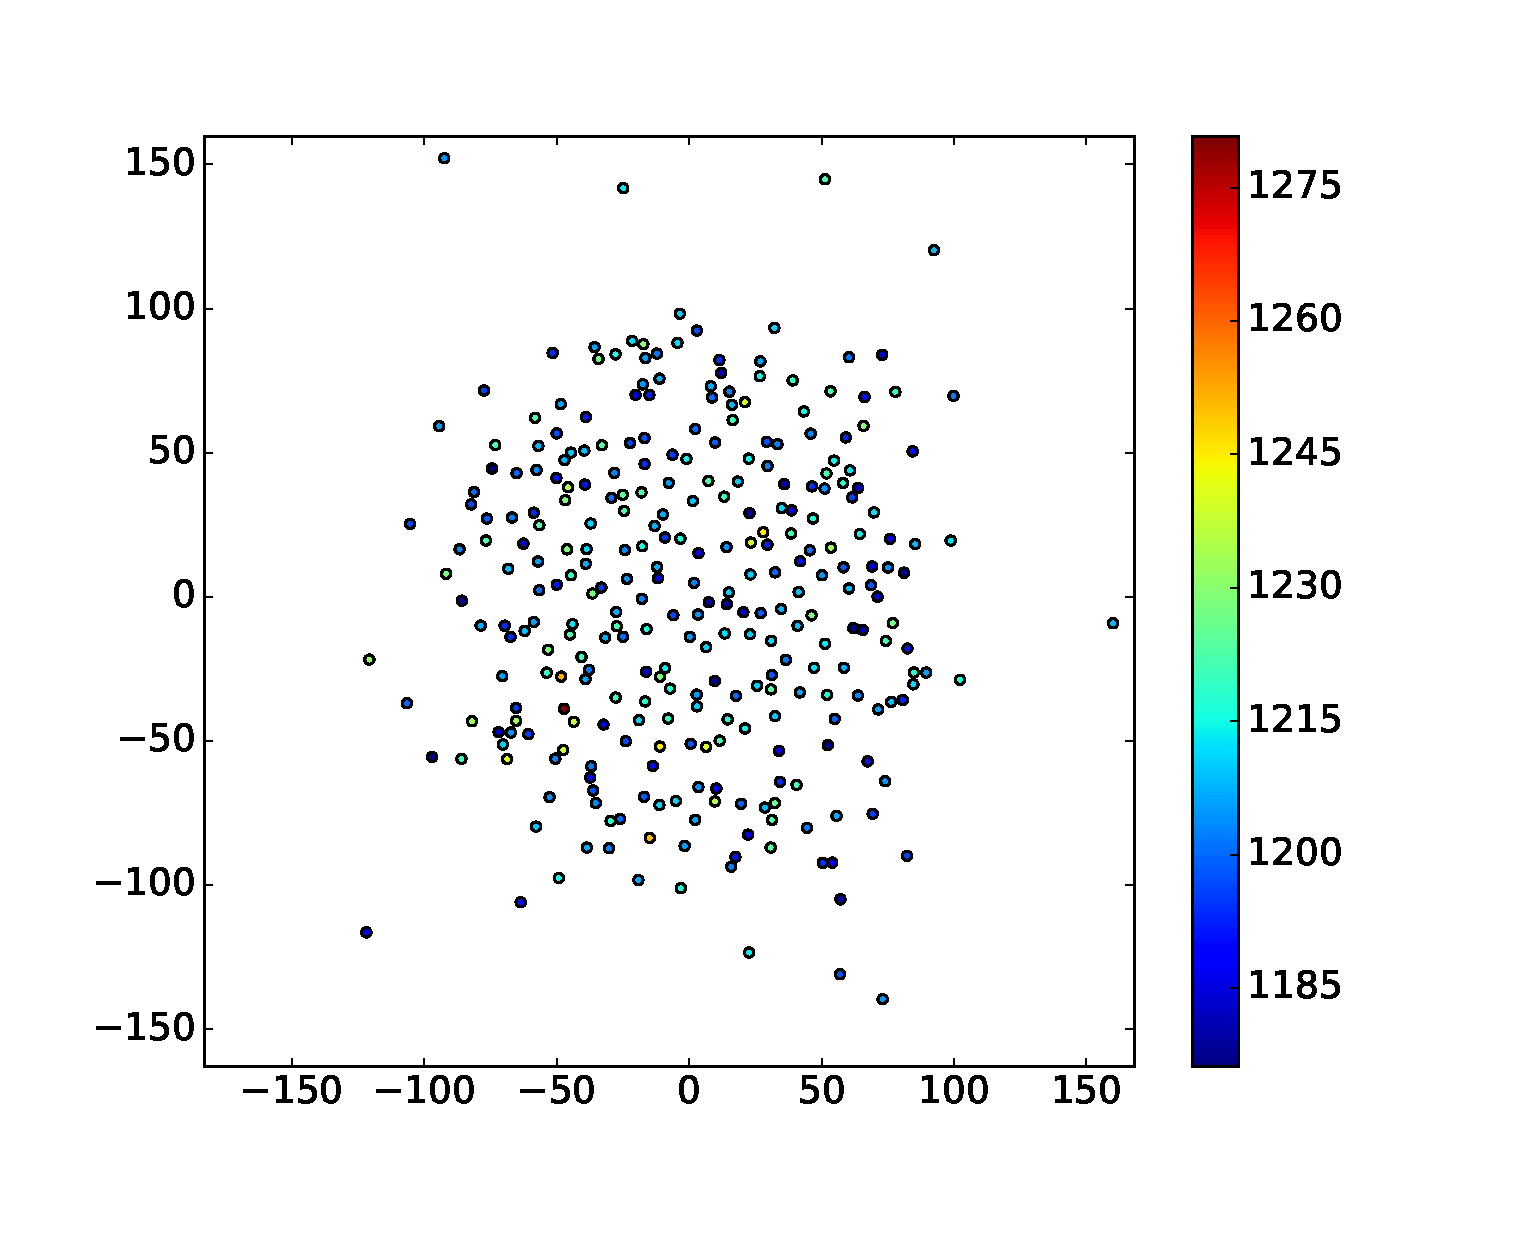
\includegraphics[width=0.5\linewidth]{presentation_pictures/plsa.eps} 
    \begin{tabular}[b]{| l | l | }\hline
      Variance MAE & $0.1$ \\ \hline
      Variance sMAPE  & $4.5 \cdot 10^{-8}$ \\ \hline
      Variance KL  & $2$ \\ \hline
      Variance KL2  & $4$ \\ \hline

      Bias MAE & $0.1$ \\ \hline
      Bias sMAPE  & $4.5 \cdot 10^{-8}$ \\ \hline
      Bias KL  & $2$ \\ \hline
      Bias KL2  & $4$ \\ \hline
    \end{tabular}

	\end{frame}
	
	
	\begin{frame}	
	\frametitle{Проверка уникальности. Initialized PLSA}
	 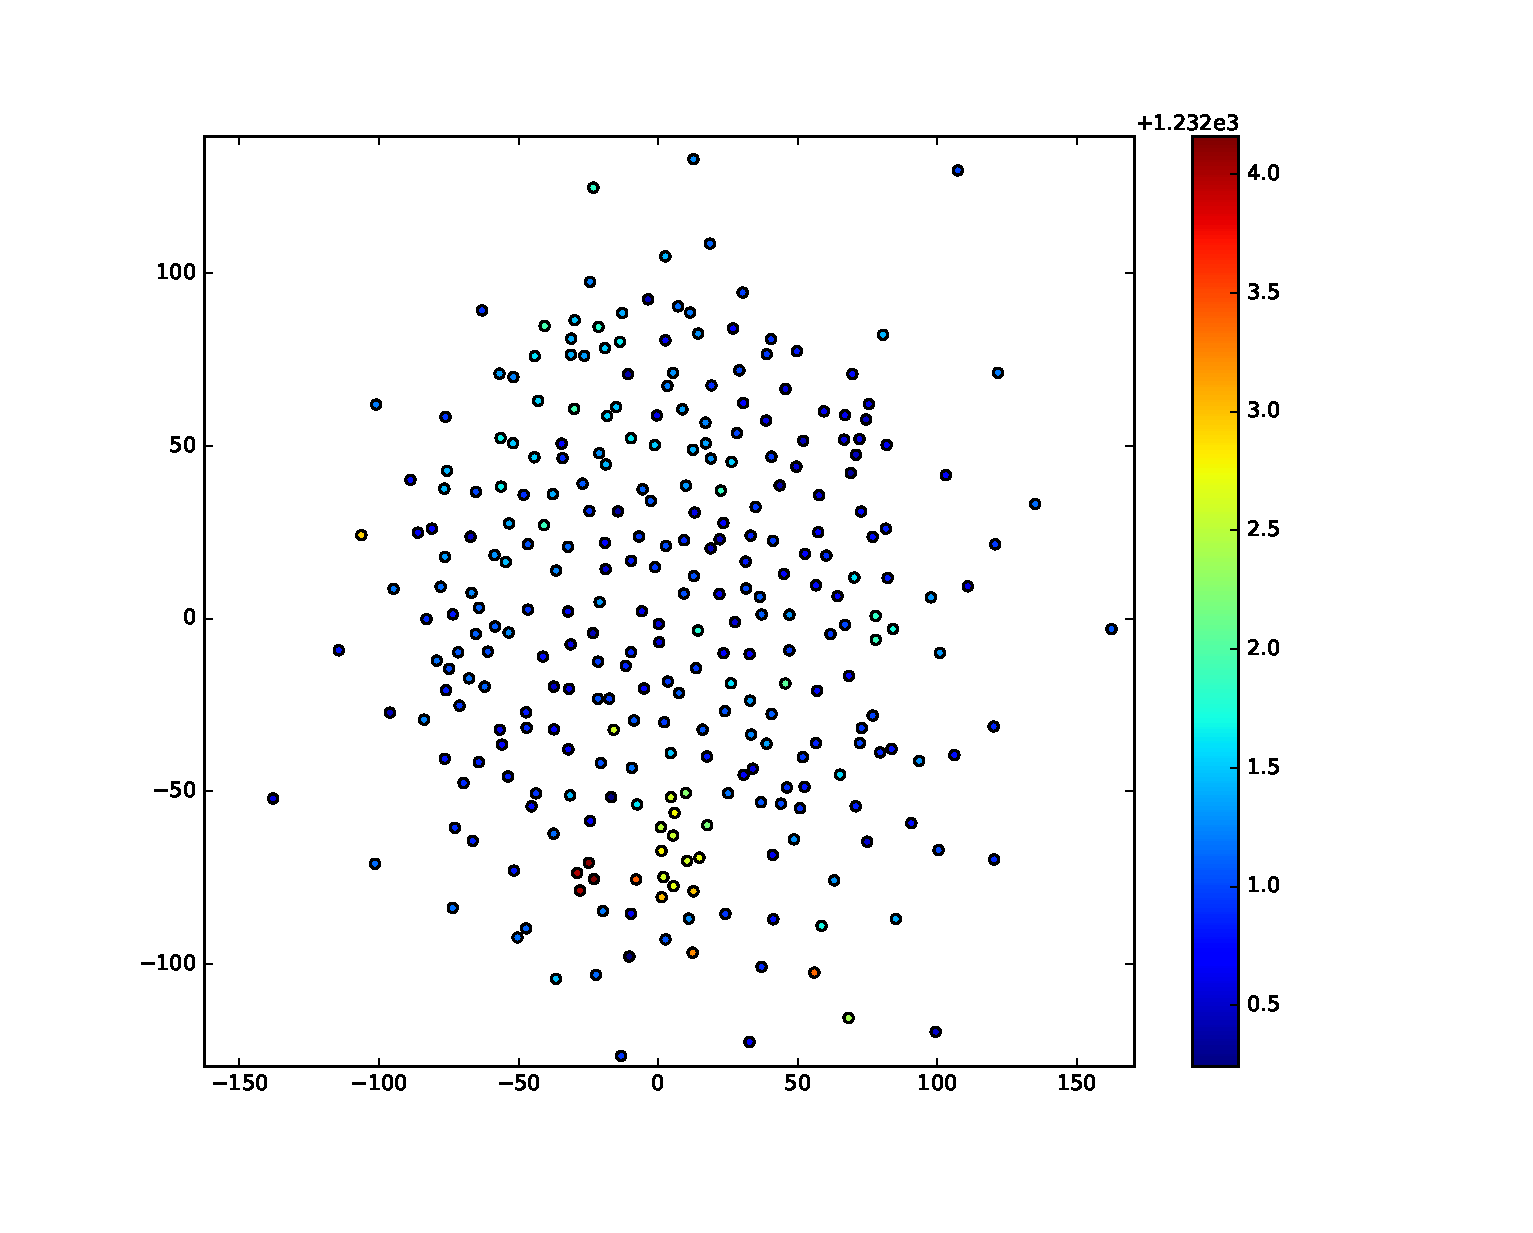
\includegraphics[width=0.5\linewidth]{presentation_pictures/full_initialized_plsa.eps} 
    \begin{tabular}[b]{| l | l | }\hline
      Variance MAE & $0.1$ \\ \hline
      Variance sMAPE  & $4.5 \cdot 10^{-8}$ \\ \hline
      Variance KL  & $2$ \\ \hline
      Variance KL2  & $4$ \\ \hline

      Bias MAE & $0.1$ \\ \hline
      Bias sMAPE  & $4.5 \cdot 10^{-8}$ \\ \hline
      Bias KL  & $2$ \\ \hline
      Bias KL2  & $4$ \\ \hline
    \end{tabular}

	\end{frame}
	
	
	\begin{frame}	
	\frametitle{Проверка уникальности. Syntetic PLSA}
	 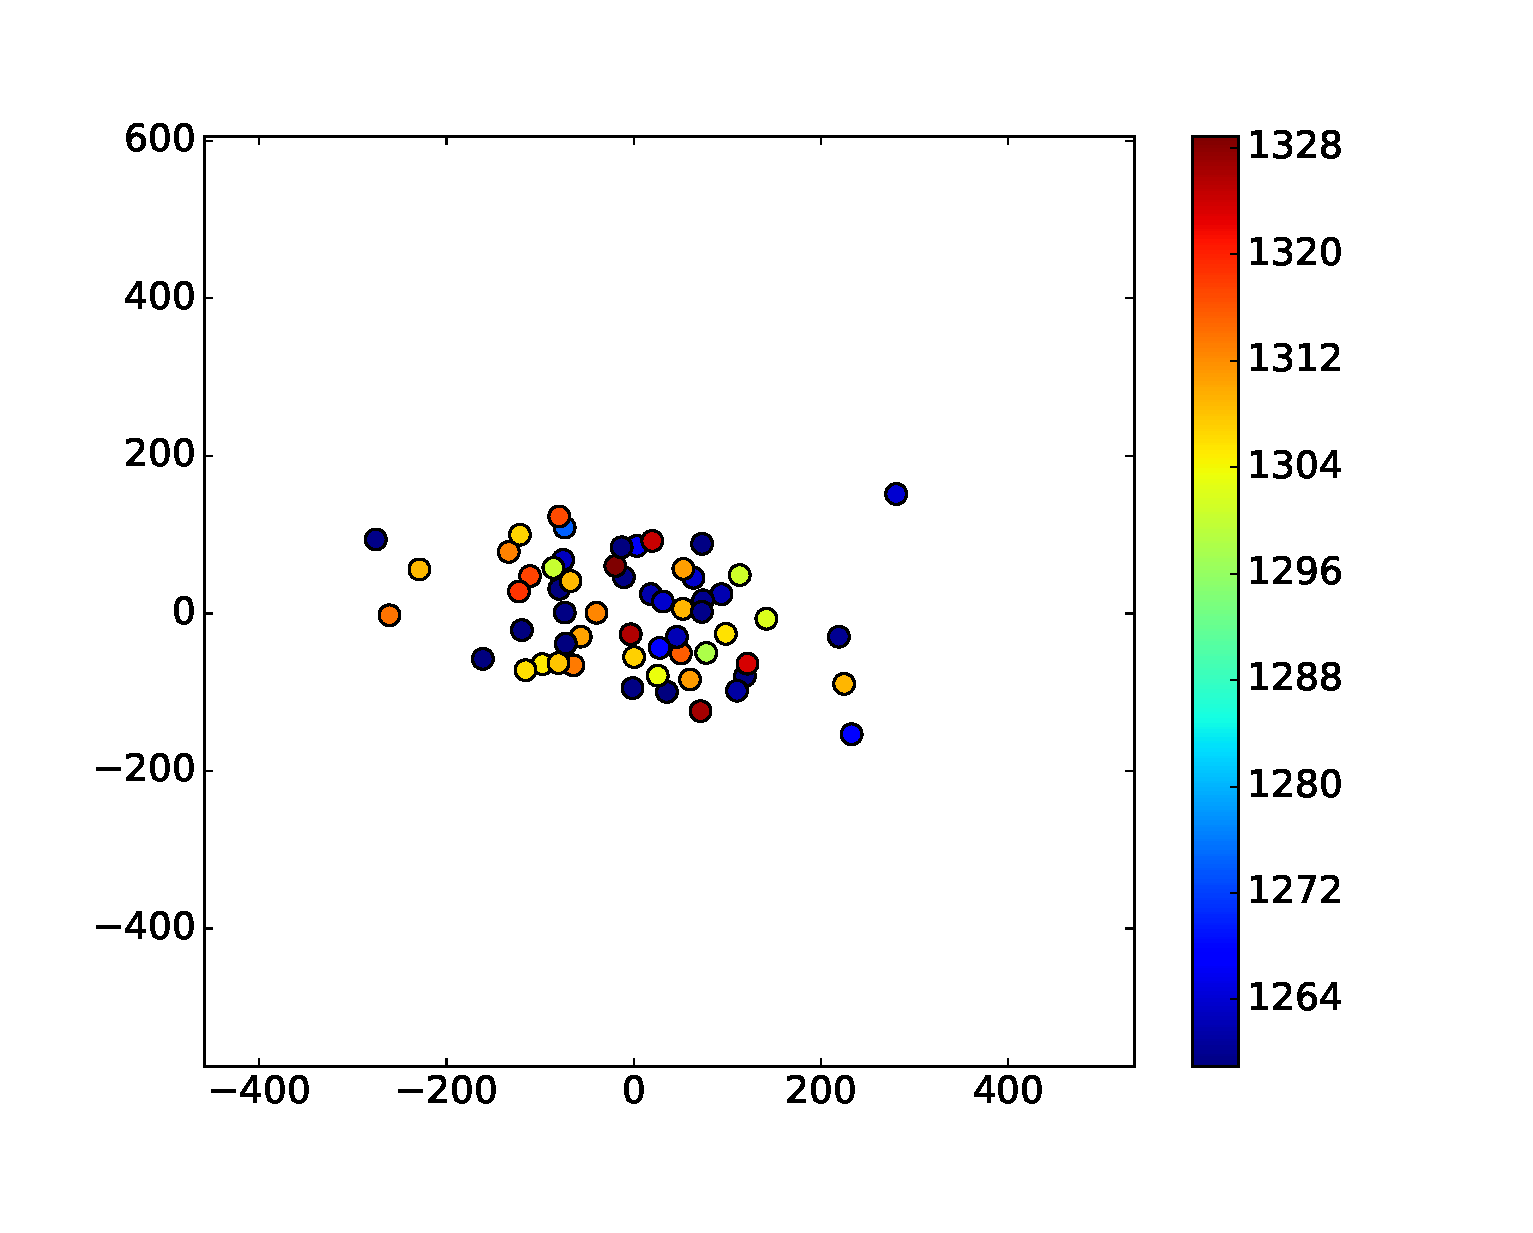
\includegraphics[width=0.5\linewidth]{presentation_pictures/syntetic_plsa.eps} 
    \begin{tabular}[b]{| l | l | }\hline
      Variance MAE & $0.1$ \\ \hline
      Variance sMAPE  & $4.5 \cdot 10^{-8}$ \\ \hline
      Variance KL  & $2$ \\ \hline
      Variance KL2  & $4$ \\ \hline

      Bias MAE & $0.1$ \\ \hline
      Bias sMAPE  & $4.5 \cdot 10^{-8}$ \\ \hline
      Bias KL  & $2$ \\ \hline
      Bias KL2  & $4$ \\ \hline
    \end{tabular}

	\end{frame}
	
	
	\begin{frame}	
	\frametitle{Проверка уникальности. Initialized Syntetic PLSA}
	 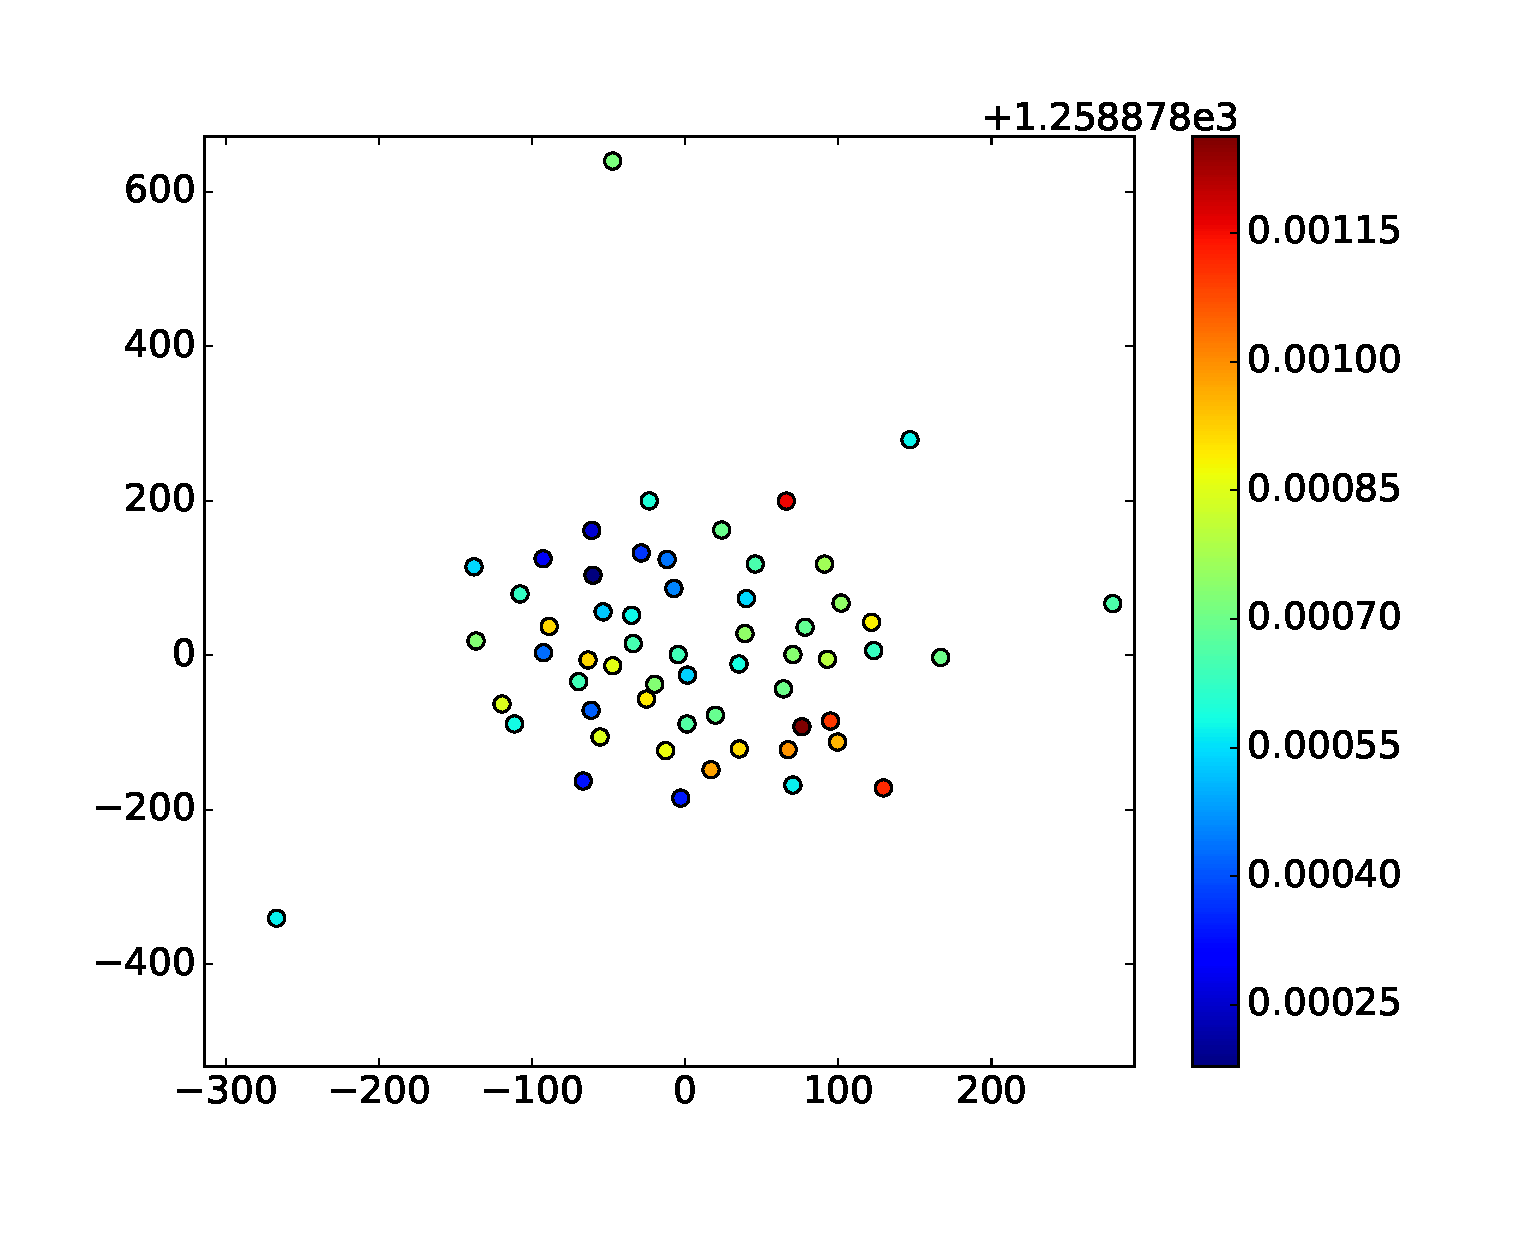
\includegraphics[width=0.5\linewidth]{presentation_pictures/full_initialized_syntetic_plsa.eps} 
    \begin{tabular}[b]{| l | l | }\hline
      Variance MAE & $0.1$ \\ \hline
      Variance sMAPE  & $4.5 \cdot 10^{-8}$ \\ \hline
      Variance KL  & $2$ \\ \hline
      Variance KL2  & $4$ \\ \hline

      Bias MAE & $0.1$ \\ \hline
      Bias sMAPE  & $4.5 \cdot 10^{-8}$ \\ \hline
      Bias KL  & $2$ \\ \hline
      Bias KL2  & $4$ \\ \hline
    \end{tabular}

	\end{frame}
	
	

\begin{frame}{Выводы}
\begin{enumerate}
\item Даже мизерного разреживания достаточно, чтобы обеспечить единственность разложения. Скорее нужно волноваться, что модель выродится, нежели станет неединственное разложение иметь.
\item Были введены две новых меры единственноости разложения. Они имеют явную связь с переобучением модели.
\item На реальных данных если фиксировать маску нулей в матрицах $\Phi$ и $\Theta$, разложение становится существенно устойчивее. Но не единственным!
\item На синтетических данных если фиксировать маску нулей в матрицах $\Phi$ и $\Theta$, разложение становится  почти единственное (колебания на уровне точности вычислений).
\end{enumerate}
\end{frame}

\end{document}
